\section{Overview and Approach}
\label{sec:overview}
\newcommand{\Motion}{\emph{Motion}\xspace}
Consider the application \LineForm in \reffig{lineform}, written in the high level programming language \lgname. \LineForm implements a simple formation control protocol of the type  used for drone shows like the one seen in \reffig{firefly}. \LineForm makes an arbitrary number of robots (drones) line up uniformly between two extremal robots. The programming tools I have built to compile and deploy \lgname code on a heterogeneous fleet of robotic platforms;
these tools can help automate the verification of these types of applications by allowing decomposition of the proofs into platform dependent and independent proof obligations. Finally, the \lgname simulator can help find violations of assumptions made for verification.

\begin{figure}[htbp!]
\centering
\begin{minipage}{0.8\linewidth}
    \begin{mdframed}
    [innertopmargin=0pt,innerbottommargin=0pt]
    \two{0.4}{0.6}
    {
        \lstinputlisting[language=NumKoord, lastline=8]{code/lineform.tex}
    }
    {
        \lstinputlisting[language=NumKoord, firstline=9, firstnumber=9]{code/lineform.tex}
    }\end{mdframed}
    \caption{\small\vspace{-4mm}\lgname program \LineForm for a set of robots to form a line.\vspace{-5mm}}
\end{minipage}

    \label{fig:lineform}
    
\end{figure}

\lgname is designed as a high-level, event-driven language in which application programs use \emph{shared variables} for coordination across robots
and \emph{ports} for interaction with hardware-specific subroutines,
In a distributed robotics setting, instances of the same \lgname program are executed by each participating robot to solve problems collectively.

\paragraph{Modules and port abstractions.}
The application programs in my design of \lgname interact with the sensors and low-level controllers of the robot platform through reads from \emph{sensor} and writes to \emph{actuator} ports(\emph{variables}).
%
%
%
For example, \LineForm uses a \emph{module} (library) called \Motion which provides a sensor port called \emph{position} that publishes the robot's position, and an actuator port called \emph{target} for specifying a target position.
%
Thus, these  ports provide an abstraction over various possible sensor and controller implementations and environments.
%
Implementations of the modules are part of the {\em Koord runtime system\/} and they implement hardware specific functions.
%, the actuator ports of different modules can be used to provide input to the controllers,
%which drives the underlying physical plant and environment.
For example, the CyPhyHouse toolchain uses an  implementation of the \Motion module for a quadcopter, relying on an indoor camera based positioning system to update the \emph{position} port,
and it uses an RRT based~\cite{lavalle1998rapidly} path planner and motion controller.
%
The \Motion module abstraction is implemented for a small racing vehicle platform using the same indoor positioning system but a different pid controller. 

\subsection{Semantics and invariant properties}

I have developed the full semantics of \lgname using \K~\cite{rosu-serbanuta-2013-k}. The execution semantics of any applications for multi-robot systems are complicated by issues of asynchrony, consistency of shared memory, and interactions between software and the physical environment. The \K rewriting engine makes the formal language semantics \emph{executable}, and enables exhaustive exploration of non-deterministic behaviors of \lgname applications.

For \LineForm, a natural requirement is to restrict all robots to stay within a certain safe area, at all times (Geofencing).
More precisely, given a (hyper)rectangle $\rect(x_{min}, x_{max})$ defined by its two corners $x_{min}$ and $x_{max}$,
if all robots are initialized within the rectangle, then all robots should always stay in the rectangle.
This requirement can be stated as:
\begin{invariant}
\label{inv:lineform}
\(
\bigwedge\limits_{i \in \UINS}
    \left(
    \begin{array}{l}
        M.pos_{i} \in \rect(x_{min}, x_{max}) \\
        \land\ x[i] \in \rect(x_{min}, x_{max})
    \end{array}
    \right)
\)
\emph{where $M.pos$ is the shorthand for $Motion.position$}.
\end{invariant}
\noindent


An invariant like the above can be established in two steps:
first, assuming that all the robot positions are in $\rect(x_{min}, x_{max})$,
we show that the targets computed by \LineForm are also in $\rect(x_{min}, x_{max})$.
The \K semantics of \lgname enables construction of the symbolic post states of the \emph{TargetUpdate} event
and prove \inv{inv:lineform} using the $\lgname$ prover (\reffig{tools}) I built. 

The second step is to show that for any robot, assuming that the computed targets are in $\rect(x_{min}, x_{max})$,
the controller implementing \Motion module indeed keeps the robot inside $\rect(x_{min}, x_{max})$.
%
For this step, one has to reason about how each robot moves when its implementation of the \Motion module is given a \emph{target}.
\lgname helps identify and decompose the overall proof into assumptions that the \emph{Module} implementations need to guarantee.

For example, one can state the key assumption needed for Invariant~\ref{inv:lineform} as:
\begin{assumption}
\label{lineform-assume}
\[
\forall t \in [0, \delta], f(M.pos, M.tgt, t) \subseteq \rect(M.pos, M.tgt),
\]
\end{assumption}
\noindent
where $M.tgt$ is the shorthand for $Motion.target$,
$f$ is a function giving the position of the robot at time $t$, moving to $M.tgt$, from $M.pos$.
This assumption states that the robot's \Motion module should ensure that it is moving within the bounding rectangle between its position and target within the duration of a round.
These types of assumptions about the control system can be discharged using verification engines for reasoning about continuous behavior of dynamical systems.

%\chiao{Give the formula representing the symbolic post or transition relation of \emph{TargetUpdate}}
%\rg{Shouldnt we postpone this to the actual section?}
\begin{figure}
\centering
\begin{tikzpicture}[
    every node/.style={draw},
]
    \node (sym) {\K Symbolic Execution};
    \node [below of=sym] (prover) {\lgname prover};
    \node [diamond, aspect=2, below of=prover] (z3) {z3};
    \node [left=1.2cm of z3] (proven) {Proven};
    \node [right=1.2cm of z3] (incon) {Inconclusive};

    \draw [->] (sym) edge (prover)
               (prover) edge (z3)
               (z3) edge node[draw=none, above, sloped] {UNSAT} (proven)
               (z3) edge node[draw=none, above, sloped] {SAT} (incon)
               ;
\end{tikzpicture}
\caption{\small \K semantics based invariant checking for \lgname.}
\label{fig:tools}
\end{figure}
\subsection{Simulation based assumption validation}

\asum{lineform-assume} may appear benign at a glance, but it may be violated in some conditions. Using the high-fidelity \lgname simulator, a designer can gain insights about when such assumptions are violated. The simulator executes complied \lgname code together with detailed physical  models for the robots, ROS-based interactions with sensor models, and UDP-based message passing.

Users can also use the simulator to detect early in the development process if the assumptions for correctness are too strong under specific scenarios, and revise the assumptions iteratively. Using the \lgname simulator in conjunction with other verification tools, one can discover that \asum{lineform-assume} is violated in three rather common scenarios:
%\chiao{Refer to simulator screenshot to show the violation.}
First, if a robot has to avoid obstacles,
then it may have to go around the obstacle and hence out of the bound.
Second, the assumption fails for robots with nonholonomic dynamics such as wheeled robots.
Third, the inertia of the robot may force it go out of bound temporarily.
\subsection{Compilation and deployment.}
In addition to the formal language, semantics, analysis, and simulation,
the complete CyPhyHouse tool chain~\cite{ghosh2019cyphyhouse} includes compilation and deployment to heterogeneous platforms including drones and race cars.
Once developers install the CyPhyHouse ROS~\cite{ros} based run-time libraries~(middleware) on a platform
and provide a device specific configuration denoting the mapping from \lgname module ports
to low level sensor and actuator ROS messages,
the port based abstraction (module) then allows the same \lgname program to run on this platform. The modular structure
 of CyPhyHouse\ {\em middleware\/} I have built will make it easy for a roboticist to add support for new hardware platforms. 
  \begin{figure*}[h!] 
    \centering
    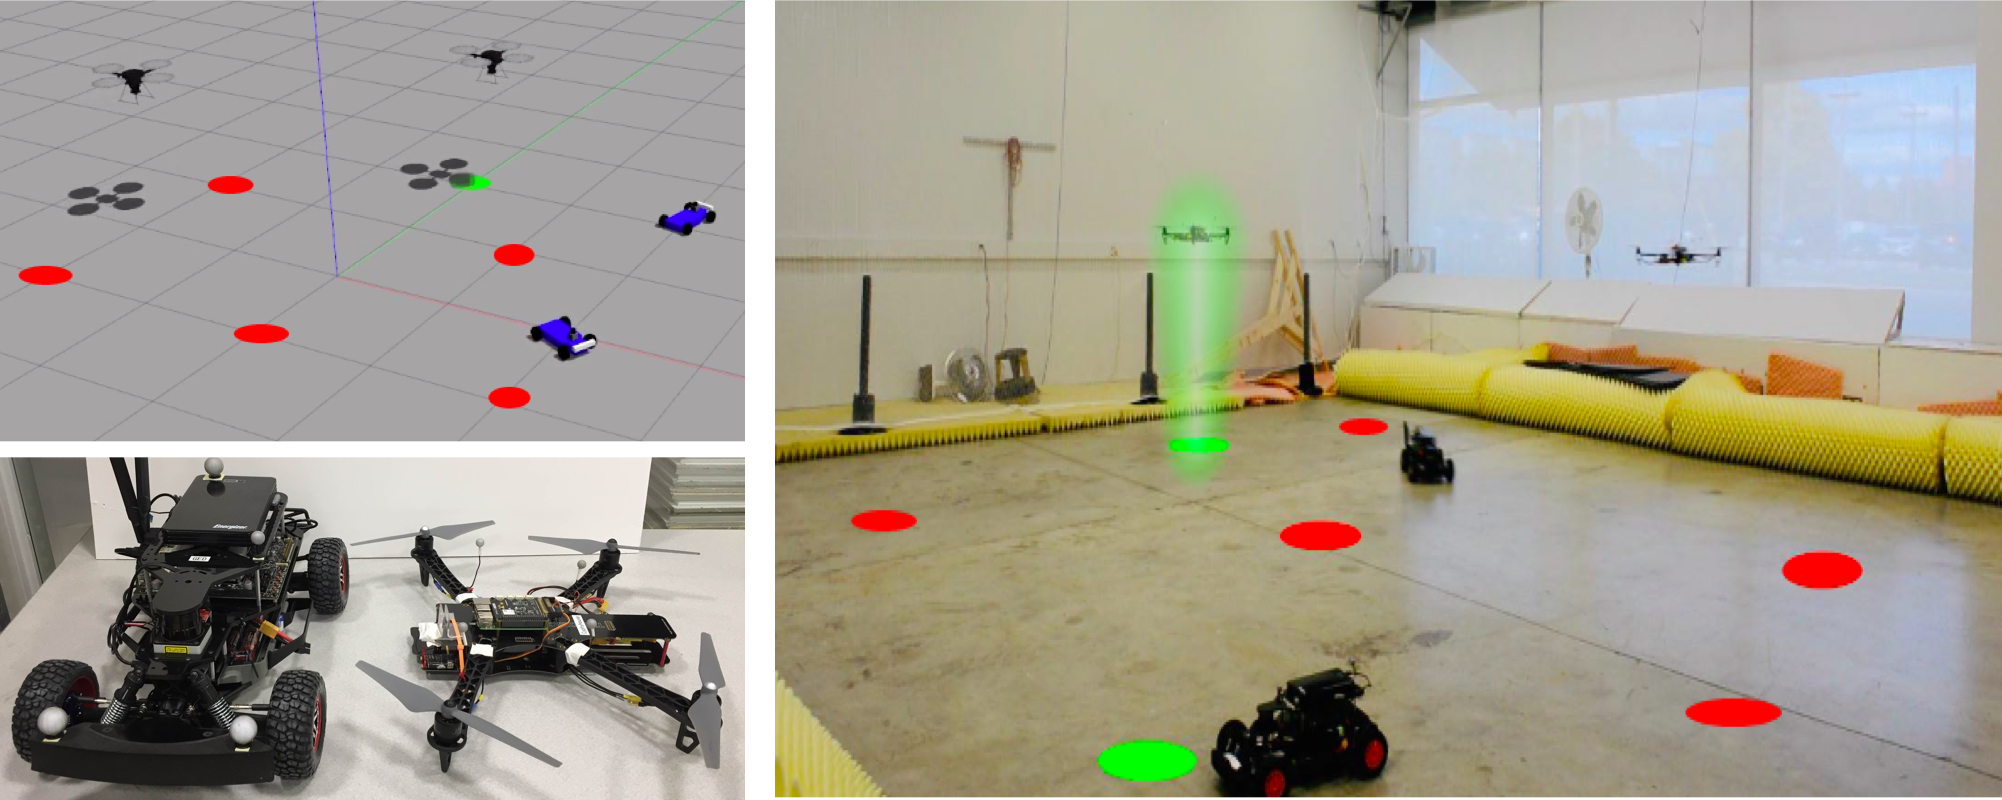
\includegraphics[width=\textwidth]{figs/irl-platform.png}
    \vspace{0.1cm}
 \caption{\small \emph{Right:} Annotated snapshot of a distributed task allocation application deployed on four cars and drones using the CyPhyHouse toolchain in the IRL test arena. The red tasks are incomplete, and the green are completed. {\em Left bottom:\/}  different robotic platforms: the F1/10 Car and the quadcopter.  \emph{Left top:\/} Visualization of the same application running in the CyPhyHouse simulator which interfaces with $\mathit{Gazebo}$.}
  \label{fig:realvis}
\end{figure*}

\subsection{Related Work}

Early domain specific languages for robotics were proprietary and tied to specific platforms. See~\cite{Nordmann2014} for a detailed survey. With the lowering hardware costs and increasing popularity, there is a growing interest in open and portable frameworks and languages~\cite{Buzzlanguage,Bohrer:2018:VVC:3192366.3192406,reactlang,williams2003model}.
%
\begin{table}[!ht]
    \footnotesize
    \centering
    \begin{tabular}{|l| c @{\hspace{0.5mm}} c @{\hspace{1mm}}c c  c @{\hspace{0.5mm}} c|}
        \hline
           \tb{Framework} & \tb{Dist.} & \tb{Hetero-} & \tb{Sim}   & \tb{Prog.}         & \tb{Compiler} & \tb{V\&V}  \\
        \tb{/system}                             & \tb{Sys.}  & \tb{geneous} &            & \tb{Lang.}         &            &            \\ \hline
        ROSBuzz~\cite{ROSBuzz}               & \checkmark & \checkmark   & \checkmark & Buzz               & \checkmark &            \\
        PythonRobotics                      &            & \checkmark   & \checkmark & Python             &            &            \\
        PyRobot~\cite{pyrobot2019}          &            & \checkmark   & \checkmark & Python             &            &            \\
        MRPT~\cite{MRPT}                     &            & \checkmark   &            & C++                &            &            \\
        Robotarium~\cite{robotarium}          &            & \checkmark   & \checkmark & Matlab             &            &            \\
        Drona~\cite{desai2017drona}           & \checkmark &              & \checkmark & P~\cite{Planguage} & \checkmark & \checkmark \\
        Live~\cite{campusanofabry:lrp2016}    &            & \checkmark   &            & LPR                & \checkmark &            \\
        \lgname                             & \checkmark & \checkmark   & \checkmark & \lgname            & \checkmark & \checkmark \\ \hline
    \end{tabular}
%            \caption{}
        \label{tab:summary}
\end{table}
%
{\em Robot Operating System (ROS)\/}~\cite{ros} is the predominant member in this category. At its core, ROS supports a publish-subscribe-based communication  and the ROS community has built drivers for  numerous hardware components.
Our implementation of the $\lgname$ abstractions for the quadcopter and vehicle platforms use ROS just like thousands of other robotics products and  projects.
 %
 The Table above gives a summary of robotics languages that have been deployed on hardware.

%\sayan{Add sentences about Drona, ROSBuzz, etc. Where is PyRobot etc in the table?}
 ROSBuzz~\cite{ROSBuzz} supports the Buzz language, which doesn't provide abstractions like $\lgname$ for path planning and shared variables. The Live Robot Programming language~\cite{campusanofabry:lrp2016} provides abstractions in terms of nested state machines and allows the program to be changed while running. It does not support robot ensembles. Programming systems using the shared memory paradigm have been developed for several distributed computing systems~\cite{dsm1991,Adve96sharedmemory,Azure,Cassandra,Dynamo}.
 %
 \sayan{A position paper~\cite{ghosh_language_2018} proposed combining shared memory with physical interactions in a high-level language. This paper presents a full language, its formalization, and the proof system that combines those abstractions.}
%
 P~\cite{Planguage} and PSync~\cite{PSyncLanguage} are DSLs for asynchronous partially distributed systems, but cyber-physical interactions are not supported. P has been integrated into the DRONA framework~\cite{desai2017drona} and the latter has very similar objectives to our work, but the approaches and solutions are different.
 In brief, DRONA abstractions, like conflict-free path planning, are more concrete and dynamics-dependent, than \lgname's abstractions. In fact, our Task application(see~\refsect{taskapp}) implements something similar to the distributed plan generator which is a built-in feature for DRONA. On the other hand, \lgname's port interfaces allow portability across arbitrary planners.


